\documentclass[a4paper,12pt]{jreport}
\usepackage{jgraduate}

\usepackage{cite}
\usepackage{url}
\usepackage{textcomp}
\usepackage{listings}
\lstset{
  frame=single,
  breaklines=true,
  numbers=left,
  language=python,
  showstringspaces=false,
  upquote=true,
}
\usepackage[dvipdfmx]{graphicx}

\title{Webアプリケーションを安全に\\するフレームワークの新しい機能}
\author{久保田 康平}
\university{九州大学}
\department{大学院システム情報科学府}
\major{情報知能工学専攻}

\date{令和 3年 2月}

\begin{document}

\maketitle

\begin{abstract}
本論文は,Webアプリケーションのセキュリティ機能向上を目的にしている.
そのために本論文では,Webアプリケーション開発者が実装するコードを実行時に自動的に解析し,必要ならば修正する機能をWebアプリケーションフレームワークに持たせることを提案し,実装して評価を行う.
Webアプリケーションはインターネットを通して世界中から誰でも接続でき,対話的に通信できるという特徴から様々な攻撃の対象になる.
また,インターネットの普及に伴いWebアプリケーションの重要性は増し,同様にWebアプリケーションの防御もまた重要になっている.
脆弱性攻撃は,Webアプリケーションの設計上の欠点や仕様上の問題点である脆弱性を利用する攻撃である.
脆弱性攻撃の対策の1つは,Webアプリケーションに脆弱性を作らないことであり,そのためWebアプリケーション開発者は一般的にWebアプリケーションフレームワーク\cite{weinberger2011systematic, bottle, flask}を利用する.
Webアプリケーションフレームワークは,Webアプリケーション開発において利用することが多いメソッドを持つライブラリである.
それらのメソッドを利用することで効率よく安全なアプリケーションを開発することができる.
セキュリティ面において,Webアプリケーションフレームワークが提供するメソッドは脆弱性対策がなされているものが多い.
したがって,Webアプリケーションフレームワークを利用した方が,利用しない時と比較して効率的にセキュアなWebアプリケーションを開発しやすい.
一方で,開発者は常に完全にセキュアなコードを書くことはできないため,Webアプリケーションフレームワークを利用して,脆弱性があるWebアプリケーションを実装してしまうことがある.
その理由の1つが,Webアプリケーション開発者がWebアプリケーションフレームワークを適切に利用できないことである.
Webアプリケーション開発者が,フレームワークのメソッドが持つセキュリティ機能を正しく理解していなかったり,
セキュリティ機能を持つメソッドを知らなかったりすることによって脆弱なWebアプリケーションが実装される.
この問題に対して本論文では,Webアプリケーション開発者が実装したソースコードを修正する機能を持つWebアプリケーションフレームワークを提案する.
提案手法を実証し評価を行った結果,この機能は実装されたコードの脆弱性を一部修正でき,レスポンスタイムは提案手法を適用しなかった場合とほとんど変わらないことを確認した.
実装された修正関数の蓄積は将来のアプリケーションのセキュリティの向上に寄与できるものである.
\end{abstract}

\tableofcontents
\listoffigures
\newpage
\pagenumbering{arabic}

\chapter{はじめに}
%目的・提案手法
本論文は,Webアプリケーションのセキュリティ機能向上を目的にしている.
その目的の達成のために,アプリケーション開発者が実装したプログラム中の関数や引数を解析し,実行時にその関数に脆弱性があった時には修正することができるWebアプリケーションフレームワークを提案,実装し評価する.

%背景(他との比較を少し入れるwaf,フレームワークのサニタイズ)
%Webアプリケーションに対する防御手法
Webアプリケーションセキュリティは,セキュリティ分野において重要である.
インターネットの普及に伴い,Webシステムは様々な場所や階層において様々な攻撃にさらされている.
Webシステムへの攻撃のうちアプリケーション層への攻撃の多くはアプリケーションのプログラムが持つ論理的な問題が原因である.
そのためWebアプリケーション開発者は攻撃を回避するために,アプリケーションの論理的な問題や設計上の欠点である脆弱性を作らない実装をする必要がある.
一方で,Webアプリケーション開発者は常にセキュアなコードを記述することはできず,脆弱性を残す実装をすることがある.
加えてWebアプリケーション層にはセキュリティに関するプロトコルや標準的な仕様がないため,Webアプリケーションの安全性は,Webアプリケーション開発者のセキュリティに関する知識や技術に依存する.
これらのWebアプリケーションの問題を解決しセキュリティを向上するために,Webアプリケーションの自動防御手法としてWebアプリケーションファイアウォール\cite{kruegel2003anomaly, epp2017anomaly, chaudhuri2010symbolic, krueger2010tokdoc, waf_ipa, ito2018web}(WAF)やWebアプリケーションフレームワーク\cite{bottle, flask, weinberger2011systematic}の利用などが検討されている.

%Webアプリケーションファイアウォール
WAFは,Webアプリケーションを脆弱性攻撃から保護するためのシステムである.
WAFはWebアプリケーションとクライアントの間に配置され,クライアントからのリクエストを監視し,リクエストが攻撃リクエストかどうかを検証する機能を持つ.
攻撃を検出した場合,そのリクエストを遮断もしくは無毒化することで,Webアプリケーションへの攻撃の影響を低減する.
WAFはWebアプリケーションを修正することなく,脆弱性攻撃を低減することが可能であるため,アプリケーションを直接修正できない時に有効な対策である.
一方でWAFはアプリケーションを修正しないので,アプリケーション内の脆弱性を根本的に修正できないという欠点がある.
またWAFはアプリケーション内の論理的な設計や仕様を知らないため,一部のタイプの脆弱性を対策することが難しい.
WAFは通常,特殊文字を含むリクエストを攻撃として検出する.
したがって,リクエスト内に特殊文字を含まない攻撃をWAFが検出することは難しい.

%Webアプリケーションフレームワーク
Webアプリケーションフレームワークは,Webアプリケーションを効率よく開発するために,Web開発に多用される機能を関数やメソッドとして提供するライブラリである.
自動防御手法としては,クロスサイトスクリプティング\cite{weinberger2011systematic}(XSS)やSQLインジェクション\cite{halfond2005amnesia}(SQLi)のようなインジェクション攻撃に対する入力検証と自動サニタイズ\cite{weinberger2011systematic}という機能を提供していることがある.
自動サニタイズとは特殊文字をエスケープする機能であるサニタイズをWebアプリケーションフレームワークが行う一部のWebアプリケーションフレームワークが持つ機能である.
自動サニタイズの長所はWebアプリケーションのセキュリティの一部をWebアプリケーションフレームワークが負担することが可能なことである.
自動サニタイズによってWebアプリケーション開発者はサニタイズについて考慮することなく,セキュアなWebアプリケーションを実装することが可能になる.
一方で自動サニタイズは限定的な対策で,インジェクション攻撃ではない攻撃を対策することが難しい.

Webアプリケーションの自動防御はWebアプリケーションの論理的な設計を検証し脆弱性の影響を低減する機能を持たないため,一部の攻撃を自動的に防御することができない.
具体的には,Webアプリケーションの不適切な認証への攻撃を自動で対策する手法をWebアプリケーションフレームワークは持たない.
不適切な認証\cite{improper_authentication}は,アプリケーションの利用者が権限を所持していると主張した時に,アプリケーションがその主張が適切かどうかを証明しない,もしくは不適切に証明する脆弱性である.

%提案手法
この問題を解決するために,本論文ではアプリケーション開発者が実装したソースコードを解析し,必要であれば修正するWebアプリケーションフレームワークであるVHF(Vulnerability Handling Framework)を提案する.
VHFは脆弱なソースコードの条件とそのソースコードを修正するプログラムを持っている.
Webアプリケーション開発者が記述したソースコードを実行開始時に静的に解析することで脆弱性を検出する.
その後,脆弱なソースコードを保護するための関数を挿入したり,安全な関数に置き換える.
挿入された関数は実行中にアプリケーションを動的に検証し,攻撃を検出すると無毒化する.
この提案手法の貢献は,Webアプリケーション開発者のソースコードを自動で修正するので,そのアプリケーションの論理的設計の不備を修正することが可能であることである.
したがってVHFは通常のWebアプリケーションフレームワークでは対策できない認証の不備に対する攻撃の低減を行うことが可能である.

%実装
VHFは実行開始時にアプリケーション開発者が実装したソースコードを修正するシステムとリクエストを処理するシステムの2つで構成されている.
ソースコードを修正するシステムはWebアプリケーション開発者が実装したソースコードを解析し修正する機能である.
VHFは実行開始時にアプリケーション開発者が実装したソースコードをフレームワーク内に格納し,その後格納したソースコードを解析・修正する.
リクエストを処理するシステムはクライアントからリクエストを受け取りレスポンスを作成して応答するシステムである.
具体的にはまず受け取ったリクエストをアプリケーションが処理しやすい形式に変更する.
次にそのリクエストを用いてレスポンスボディを作成する.
最後にレスポンスを作成する.
リクエストに基づいてレスポンスヘッダーを作成し,レスポンスボディと組み合わせてレスポンスを作成する.
作成されたレスポンスはクライアントに返される.

%評価
本論文ではWebアプリケーション開発者が実装したソースコードを解析して脆弱性の影響を緩和することが可能であるかを確認するために実験を行った.
その結果,不適切な認証とSQLiの脆弱性を修正できることを確認した.

\chapter{関連研究}
\section{論文1}
\section{論文2}
\section{論文3}

\chapter{提案手法}
この章では,コールバック関数を解析し必要であれば修正するWebアプリケーションフレームワークであるVHFを提案する.
コールバック関数とはWebアプリケーションへのリクエストを基に,Webサーバー側で行う処理を記述した関数である.
図\ref{fig:vhf}はVHFを利用したWebアプリケーションの概要図である.
\begin{figure}[ht]
  \begin{center}
    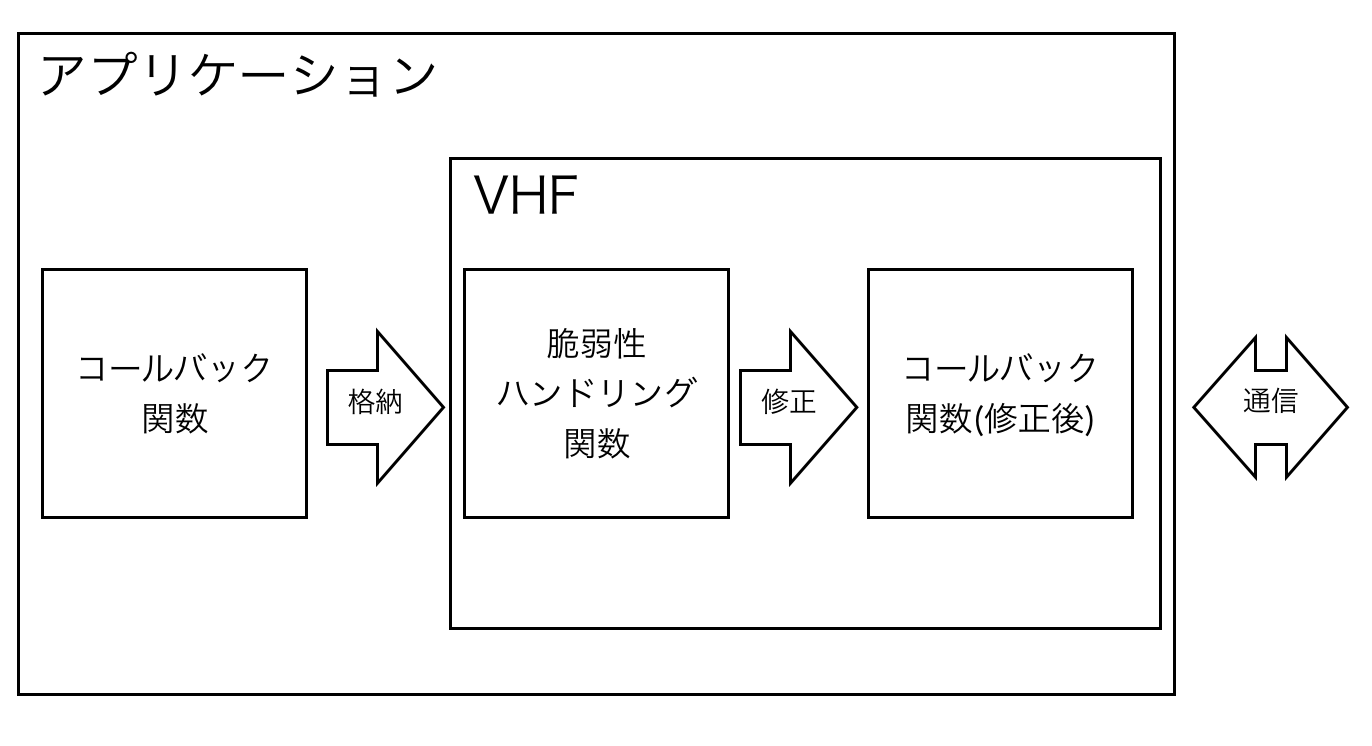
\includegraphics[clip, width=130mm]{./figures/vhf.png}
    \caption{VHFの概要図}
    \label{fig:vhf}
  \end{center}
\end{figure}
VHFはコールバック関数の修正機能とリクエストの処理機能を持っている.
VHFが実行されるとまずコールバック関数を修正する.
具体的には実行開始時にVHFはコールバック関数をVHF内に格納し,コールバック関数を修正する.
その後実行中はクライアントからのリクエストに対して修正されたコールバック関数で処理を行うことで脆弱性の影響を低減する.

VHFはサイバーセキュリティの観点から3つの利点がある.
まず1つ目にVHFが対策しているコールバック関数に関するセキュリティ機能の全てをアプリケーション開発者が負担しなくていい点である.
一般的なWebアプリケーションフレームワークにおけるWebアプリケーションの実装では,Webアプリケーション開発者は安全なコールバック関数を実装する全責任を負っている.
VHFはコールバック関数を自動で解析・修正するので,VHFがコールバック関数の責任の一部を担うことが可能である.
第2に,VHFはWAFで対策が難しい脆弱性攻撃を対策可能である.
一般的なWAFはアプリケーションへのリクエストを解析することで脆弱性攻撃の影響を低減する.
具体的には,リクエスト中の特殊文字や他のプログラミング言語に関する意味のある文字を脆弱性攻撃としそれらを検出する.
この検出手法はWebアプリケーションを修正することなくWebアプリケーションを自動で防御できるが,リクエスト中に特殊文字を含まない攻撃を対策することが困難である.
リクエスト中に特殊文字を含まない攻撃の1つが不適切な認証を持つアプリケーションへの攻撃である.
不適切な認証は,Webアプリケーションの論理的な設計の間違いが原因で起こる脆弱性である.
不適切な認証によって正しいアクセス制御ができず,それにより特権を持たないユーザーが特権リソースに接続する攻撃が発生する.
VHFはコールバック関数間の論理的な設計を比較して他のコールバック関数に適用することで不適切な認証の影響を低減することが可能である.
第3に,VHFはコールバック関数を実行開始時に修正するので脆弱性を根本的に対策することが可能である.
WAFは,コールバック関数の脆弱性を削除できないため,特定の攻撃を対策してもその対策を迂回する攻撃が発生する可能性がある.

VHFは図\ref{fig:4steps}に示す通り,実行開始時に4つの工程によってコールバック関数を解析・修正する.
図\ref{fig:4steps}の上部はコールバック関数の形式であり,下部がVHF内部で行われる工程である.
\begin{figure}[ht]
 \begin{center}
  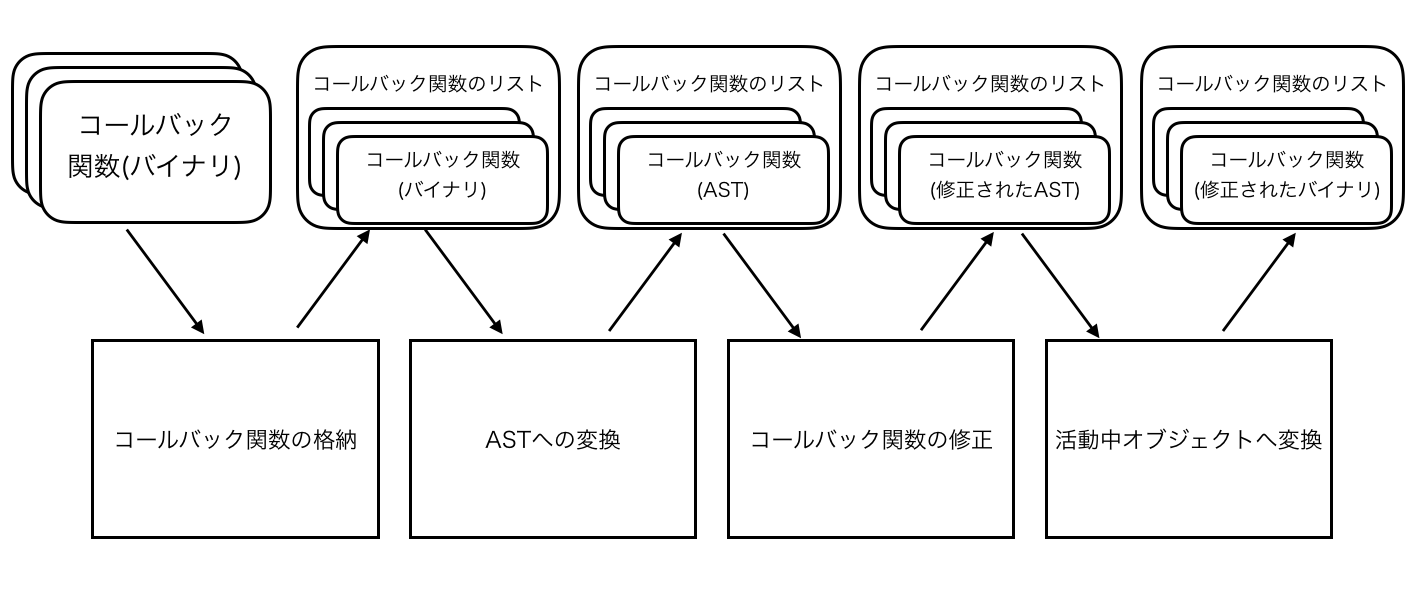
\includegraphics[clip, width=130mm]{./figures/4steps.png}
  \caption{コールバック関数を修正するための4つの工程}
  \label{fig:4steps}
 \end{center}
\end{figure}
まず最初に,コールバック関数,リクエストパス,メソッドを1つの辞書式データとしてVHFに格納する.
この辞書式データはリストの一要素としてVHFに格納される.
この時点ではコールバック関数は活動中のオブジェクト,つまり実行可能なバイナリ形式のオブジェクトである.
次にコールバック関数を修正しやすくするために,VHFはコールバック関数の形式を活動中のオブジェクトから抽象構文木\cite{ref:ast}(Abstract Syntax Tree: AST)に変更する.
ASTは,プログラムを実行可能なバイナリ状態にする処理の途中で取得される中間生成物であり,ソースコードから実行可能なオブジェクトを生成するために必要ない部分を削除した表現である.
ASTはバイナリよりもプログラムの論理的設計を把握しやすいため,コールバック関数の解析と修正が容易である.
\begin{figure}[t]
 \begin{center}
  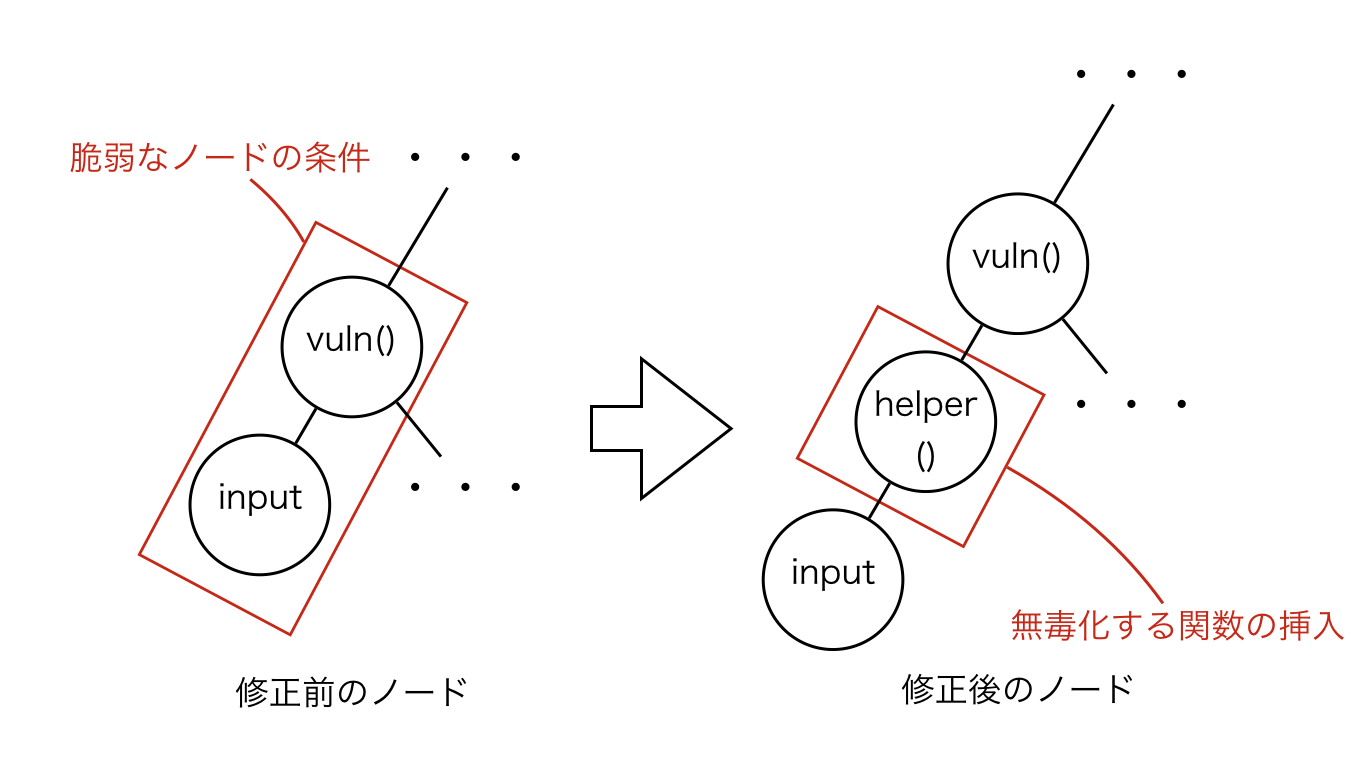
\includegraphics[clip, width=130mm]{./figures/modifying_ast.png}
  \caption{ASTの修正による脆弱性影響低減手法の概要図}
  \label{fig:modifying_ast}
 \end{center}
\end{figure}
3つ目がコールバック関数の解析と修正である.
VHFはコールバック関数を解析し修正する脆弱性ハンドリング関数を持っている.
脆弱性ハンドリング関数は特定の属性と名前を持つノードを脆弱なノードとし,このノードを再帰的に探索して検出して,その後脆弱性ハンドリング関数の処理によってノードの一部を修正される.
具体的な修正方法は,脆弱なノードにVHFが持つ関数やメソッドを挿入する.
脆弱性ハンドリング関数は図\ref{fig:modifying_ast}に示すように,脆弱なノードの一部に攻撃を無毒化する関数を挿入することで,実行時に変数を動的に検証し,攻撃を無毒化する.
図\ref{fig:modifying_ast}では,vuln()関数を脆弱なノードの条件としており,vuln()関数の引数inputを無毒化する関数helper()を挿入することで,脆弱性の影響を低減している.
脆弱性ハンドリング関数はコールバック関数のリストを引数として受け取る.
このリストは全てのコールバック関数がASTの状態で格納されている.
脆弱性ハンドリング関数は全てのコールバック関数を受け取ることで,単一のコールバック関数内の脆弱性だけでなく,コールバック関数間の論理的な設計によって起きる脆弱性を対策することが可能である.
脆弱性ハンドリング関数はコールバック関数を修正したのち,全てのコールバック関数が格納されたリストを返す.
最後に,修正されたコールバック関数のASTを実行可能なオブジェクトに戻す.
実行可能な状態になった修正されたコールバック関数は,クライアントの通信の際に呼び出されリクエストを処理することができる.

\chapter{実装}
この章では,VHFの実装について記述する.
VHFはPython3.7によって実装されている.
VHFは2つのシステムによって構成されている.
コールバック関数を修正するシステムとリクエストを処理するシステムである.
実行開始時にコールバック関数を修正するシステムにより,コールバック関数が修正され,実行中はクライアントのリクエストに基づきレスポンスを返す.

\section{コールバック関数の修正機能}
VHFは実行開始時にコールバック関数を解析・修正する.
この時にコールバック関数の格納,コールバック関数のASTへの変換,コールバック関数の修正,コールバック関数の活動中のオブジェクトへの変換が行われる.
それぞれの実装について下に記述する.

\subsection{コールバック関数の格納}
VHFはコールバック関数を格納するためにデコレータを利用するためのメソッドとしてrouteメソッドを持つ.
実効開始時にrouteメソッドはコールバック関数をVHF内のリストに格納する.
以下のソースコードはコールバック関数の例である.
\begin{lstlisting}[caption={コールバック関数の一例}, label=code:callback, captionpos=b]
@app.route(path='^/$', method='GET')
def index(request):
  return "Hello"
\end{lstlisting}
ソースコード\ref{code:callback}の1行目がデコレータである.
デコレータは関数を修飾する関数であり,下記のソースコード\ref{code:callback2}はソースコード\ref{code:callback}と糖衣構文である.
デコレータを利用することで関数を引数にする関数の記述を簡易にしてくれる.
\begin{lstlisting}[caption={ソースコード\ref{code:callback}と糖衣な表現}, label=code:callback2, captionpos=b]
def index(request):
  return "Hello"
index = app.route(path="/", method="GET")(index)
\end{lstlisting}
ソースコード\ref{code:callback}の1行目にあるappはVHFのモジュールであり,routeはappモジュールが持つメソッドの1つである.
routeメソッドはリクエストパスとリクエストメソッドを引数としている.
ソースコード\ref{code:callback}のpathがリクエストパスの正規表現,methodがリクエストメソッド,2行目と3行目の関数が第3引数のコールバック関数である.
コールバック関数はrequestを引数として受け取る.
requestはリクエストの情報を格納している変数である.
ソースコード\ref{code:callback}の3行目は戻り値であり,この戻り値はその後レスポンスボディになる.
routeメソッドはリクエストパスとリクエストメソッドをコールバック関数と対応付けてVHFに格納する.
以下のソースコード\ref{code:route_method}がrouteメソッドの実装である.
\begin{lstlisting}[caption={routeメソッド}, label=code:route_method, captionpos=b]
class App():
  ...
    def route(self, path=None, method='GET'):
        def decorator(callback_func):
            self.router.add(method, path, callback_func)
            return callback_func
        return decorator
\end{lstlisting}
routeメソッドを実行するとrouteメソッド内部のdecorator関数を返す.
その後コールバック関数を引数としたdecorator関数が実行される.
decorator関数内のrouter.addメソッドはコールバック関数をVHFに格納するメソッドである.
decorator関数はコールバック関数とリクエストパス,リクエストメソッドの要素を持つ辞書形式にして,その辞書データをリストに格納する.

\subsection{コールバック関数のASTへの変換}
VHFに格納された時点ではコールバック関数は活動中のオブジェクト,つまり機械語である.
機械語を解析・修正するのは容易ではないため格納されたコードを一度修正しやすい形式に変換する.
具体的には,活動中のオブジェクトをASTに変換する.
Pythonは活動中のオブジェクトをASTに直接変換できないため,活動中のオブジェクトを一度ソースコードに変換したのちにASTに変換する.
活動中のオブジェクトからソースコードを取得するために,Pythonが提供しているinspectモジュールのgetsourceメソッドによりソースコードを取得する.
getsourceメソッドは活動中のオブジェクトを引数に取り,そのソースコードを返すメソッドである.
Pythonの活動中オブジェクトは関数名やソースコードのファイルのパスなどの情報を保持している.
その情報を利用してgetsourceメソッドはソースコードのファイルを読み取り,ソースコードを取得する.
動的に実行された活動中のオブジェクトには,ソースコードのファイルなどの情報がないため,getsourceメソッドでソースコードを取得できない点には注意が必要である.
getsourceメソッドが取得したソースコードはrouteデコレータを含むため,そのままASTに変換できない.
そのため,コールバック関数の先頭にあるrouteデコレータを取得したソースコードから取り除く.
その後,取得したソースコードをASTに変換する.
Pythonは,ASTを処理するライブラリとしてastモジュールを提供している.
このモジュールは,ソースコードをASTに変換したりASTを探索したりするメソッドを持っている.
parseメソッドはastモジュール内にある,ソースコードをASTに変換するメソッドである.
parseメソッドはソースコードを引数として受け取るため,格納された時点での活動中のオブジェクトとしてのコールバック関数を受け取ることはできない.
したがって,一度コールバック関数をソースコードに変換したのち,parseメソッドを利用してコールバック関数をソースコードからASTに変換する.
生成されたASTは,リクエストメソッドとリクエストパス,ASTを要素とする辞書形式にまとめられ,この辞書型式のデータはリストに格納される.

\subsection{コールバック関数の修正}
その後VHFはASTになったコールバック関数を解析・修正する.
VHFはコールバック関数を修正する関数として脆弱性ハンドリング関数を実装している.
脆弱性ハンドリング関数はASTであるコールバック関数のリストを引数に取り,解析・修正されたASTであるコールバック関数のリストを返す.
脆弱性ハンドリング関数の内部では脆弱性と判断したノードがコールバック関数内にあるかを解析し,検出されたノードを脆弱性ハンドリング関数内で定義したノードの修正方法に基づいて修正する.

脆弱性ハンドリング関数は新しい脆弱性が発見された時に追加の実装をしやすくするために脆弱性ハンドリング関数を分割している.
脆弱性ハンドリング関数は脆弱性ごとに分割されており,これらの分割された脆弱性ハンドリング関数はリストに格納される.
コールバック関数のリストは図\ref{fig:vh_funcs}に示すように順に脆弱性ハンドリング関数によって解析・修正される.
%図
\begin{figure}[ht]
  \begin{center}
    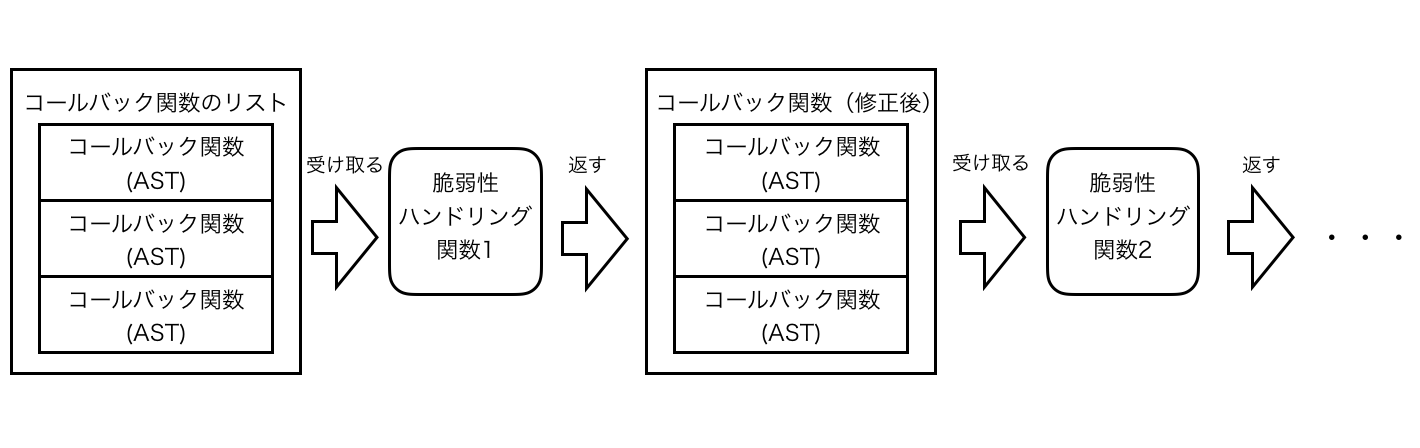
\includegraphics[clip, width=130mm]{./figures/splited_vhfunction.png}
    \caption{脆弱性ハンドリング関数がコールバック関数を修正する概略図}
    \label{fig:vh_funcs}
  \end{center}
\end{figure}

\subsection{コールバック関数の活動中のオブジェクトへの変換}
最後にコールバック関数を活動中のオブジェクトに変更する.
ASTを実行可能な形式に変更するために,exec()関数を利用する.
これにより,コールバック関数は活動中のオブジェクトとなり,リクエストを処理することが可能になる.

\section{リクエスト処理システム}
リクエスト処理システムはリクエストを基にコールバック関数を呼び出しレスポンスを作成するシステムである.
このシステムはリクエスト情報の取得,コールバック関数の呼び出し,リクエストの作成の3つの工程でリクエストを処理する.

\subsection{リクエスト情報の取得}
リクエスト情報の取得は,クライアントからのHTTPリクエストを取得し,アプリケーションが処理しやすいように加工する工程である.
この工程ではrequestインスタンスが作成される
具体的には,リクエストパラメータを辞書形式に変換したり,リクエストボディをしたりして,HTTPリクエストを元にrequestインスタンスを作成する.
requestインスタンスのインスタンス変数がリクエスト情報になる.
例えばrequest.pathがリクエストパス,request.methodがリクエストのメソッド,request.queryがリクエストのパラメータである.
このインスタンス変数はコールバック関数に引数として与えられる.

\subsection{コールバック関数の呼び出し}
リクエストパスとリクエストメソッドに基づき,コールバック関数を呼び出しレスポンスボディを作成する.
VHFに格納されている修正されたコールバック関数のリストから,リクエストパスとリクエストメソッドが一致するコールバック関数を探す.
一致するコールバック関数が存在する場合,requstを引数に与えてコールバック関数を実行する.
コールバック関数の戻り値がレスポンスボディに相当する.
一方,一致するコールバック関数がない場合,「Not Found」をレスポンスボディにする.

\subsection{レスポンスの作成}
レスポンスボディをエンコードし,レスポンスヘッダーを作成したのち,レスポンスヘッダーとレスポンスボディを組み合わせレスポンスを作成する.
一致するコールバック関数が存在しレスポンスボディが作成された時は,レスポンスヘッダーのステータスコードを200,存在しない時は404とする.
レスポンスヘッダーとレスポンスボディを組み合わせクライアントに送信する.

\chapter{実験}
VHFについて2つの実験を行った.
1つ目に脆弱性ハンドリング関数が脆弱性の影響を低減したかどうかの評価を行った.
2つ目に脆弱性ハンドリング関数が実装されたことによる実行開始時のオーバーヘッドの計測を行った.
本実験は以下の環境で行われた.
Mac OS X El Capitan 10.11.6, Intel Core i5(2.95GHz), メインメモリ8GBであった.

\section{脆弱性の影響低減評価実験}
脆弱性ハンドリング関数を実装することにより脆弱なコールバック関数を修正し,脆弱性攻撃への影響を低減することが可能か評価した.
本実験では2つの脆弱性を持つアプリケーションを1つ実装した.
実装されたアプリケーションが持つ2つの脆弱性はSQLiと不適切な認証である.
この脆弱性に対して,それぞれ脆弱性ハンドリング関数を実装した.
その後,ローカル上でアプリケーションを実行し,攻撃することで脆弱性攻撃の影響を低減できたか評価した.
以下には,それぞれの脆弱なコールバック関数と脆弱性ハンドリング関数を記述する.

\subsection{SQLiを持つコールバック関数の修正と攻撃}
SQLiはリクエスト内の値を利用して直接クエリを作成することで起こる脆弱性である.
リクエストに特殊文字を挿入することで,アプリケーション開発者が意図していない命令がデータベースで実行される.
これにより,データベースが改ざんされたり不正に削除されたりする.
本実験では,以下の図に示すようにSQLi脆弱性を持つアプリケーションが実装された.
%図
%図の説明userテーブルを持っていることを説明
下記のソースコード\ref{code:sqli_callback}はSQLi脆弱性を持つアプリケーションのコールバック関数の一部である.
\begin{lstlisting}[caption={SQLi脆弱性を持つコールバック関数}, label=code:sqli_callback, captionpos=b]
@app.route("^/access$", "POST")
def access(request):
  import sqlite3
  conn = sqlite3.connect("test.sqlite3")
  cur = conn.cursor()
  action = request.forms.get('action')
  name = request.forms.get('name')
  password = request.forms.get('password')
  query = '{action} * from user'.format(action=action)
  if action='select':
    query += " where name = '{name}' and password = 'password'".format(name=name, password=password)
    cur.execute(query)
    data = cur.fetchone()
    return tmpl("access.html", action='select',tel=data[2],mail_address=data[3])
  else:
    cur.execute(query)
  return tmpl("access.html", action=action)
\end{lstlisting}
上記のソースコード\ref{code:sqli_callback}は,リクエストパラメータに基づいてデータベースを操作し,その結果をクライアントに返すコールバック関数である.
このソースコードの1行目は,コールバック関数を格納するメソッドである.
リクエストパスが"/access"でリクエストメソッドがPOSTの時,このコールバック関数が呼び出される.
2行目以降のaccess()関数がコールバック関数である.
ソースコード\ref{code:sqli_callback}の3行目から5行目でデータベースと接続する準備をしている.
3行目でリレーショナルデータベースとしてsqlite3をインポートしている.
4行目でデータベースに接続し,5行目でカーソルを宣言している.
その後ソースコード\ref{code:sqli_callback}の6行目から8行目では,クエリを作成するために必要な情報をリクエストパラメータから取り出している.
取り出される変数はaction, name, passwordである.
actionはSQLのコマンド,nameはユーザー名,passwordはユーザーのパスワードである.
ソースコード\ref{code:sqli_callback}の9行目と11行目でこれらの変数を利用してクエリを作成する.
ソースコード\ref{code:sqli_callback}の12行目で作成したクエリがデータベースで実行される.
上記のソースコード\ref{code:sqli_callback}は,リクエストパラメータを直接利用してクエリを作成しているためSQLi脆弱性を持っている.

このソースコードに対して,クエリを実行するコードを修正する脆弱性ハンドリング関数を実装した.
この脆弱性ハンドリング関数はcurインスタンスのexecuteメソッドが持つ引数をエスケープするescape\_special\_query()関数を挿入した.
escape\_special\_query()関数はクエリを引数に取りクエリにdrop命令が入っている場合クエリを捨てる関数である.
上記ソースコードでは\ref{code:sqli_callback}の12行目と16行目のcur.execute()メソッドの引数をescape\_special\_query()関数でエスケープした.
%図
結果として,上図に示すようにソースコードは変更された.
下記のソースコード\ref{code:sqli_handling}は実装された脆弱性ハンドリング関数の一部である.
\begin{lstlisting}[caption={SQLiの影響を低減するための脆弱性ハンドリング関数の一部}, label=code:sqli_handling, captionpos=b]
class InsertQueryChecker(ast.NodeTransformer):
  def visit_Call(self, node):
    if isinstance(node.func, ast.Attribute):
      if isinstance(node.func.value, ast.Name):
        if node.func.value.id is 'cur':
          if node.func.attr is 'execute':
            new_args = []
              for arg in node.args:
                new_arg = ast.Call(
                  func=(ast.Name(id='escape_special_query', ctx=ast.Load())),
                    args=[arg],
                    keywords=[]
                  )
                new_args.append(new_arg)
                new_node = ast.Call(
                  func=node.func,
                  args=new_args,
                  keywords=node.keywords
                )
              return ast.copy_location(new_node, node)
    return node
\end{lstlisting}
ソースコード\ref{code:sqli_handling}の1行目は,クラスの宣言である.
ast.NodeTransformerクラスはASTを再帰的に探索するastモジュールが持つクラスである.
このクラスのvisit\_属性というメソッドは特定のノードを検出した時に実行されるメソッドであり,ソースコード\ref{code:sqli_handling}の2行目のvisit\_Call()メソッドはノードの属性がast.Callの時に実行されるメソッドである.
ソースコード3行目から6行目がcur.execute()メソッドを検出するノードの条件である.
その後条件に一致するASTを検出し,ソースコード\ref{code:sqli_handling}の9行目から19行目でASTを修正する.

脆弱性ハンドリング関数によって脆弱性の影響を低減できたか確認するために,まず脆弱性ハンドリング関数の実行部分をコメントアウトしたアプリケーションでローカル上の8000番ポート実行し,このアプリケーションに対して攻撃を行った.
次に,脆弱性ハンドリング関数に解析・修正されたアプリケーションをローカル上の8000番ポートに立ち上げ,攻撃であるリクエストをアプリケーションに送信した.
攻撃リクエストはパスが/loginで,クエリの要素となるリクエストボディ部分がaction=drop user;-\--\&id=name\&password=passwordとした.

\subsection{不適切な認証を持つコールバック関数の修正と攻撃}
不適切な認証を持つコールバック関数をVHF上に実装した.
このコールバック関数は図に示すように/loginへのリクエストでは認証を行い,アプリケーション内に登録されたユーザーは"ADMIN\_PAGE"が返却される.
一方,/homeへのリクエストは,認証なしに"ADMIN\_PAGE"を返却する.
このコールバック関数は適切に認証を行っていないため,全てのユーザーが"ADMIN\_PAGE"を閲覧可能である.
"ADMIN\_PAGE"が権限を必要とするページである時,このアプリケーションは不適切な認証の脆弱性を持つ.
以下のソースコード\ref{code:auth_leak_callback}が実装したコールバック関数である.
\begin{lstlisting}[caption={A vulnerable function which has an authentication leak.}, label=code:auth_leak_callback, captionpos=b]
@app.route("^/login$", "POST")
def do_login(request):
    id = request.params["ID"]
    password = request.paramas["PASSWORD"]
    if is_admin(id, password):
        return "ADMIN_PAGE"
    else:
        return "LOGIN_PAGE"

@app.route("^/home$", "GET")
def home(request):
    return "ADMIN_PAGE"
\end{lstlisting}

このアプリケーションには2つのコールバック関数が実装された.
1つ目がdo\_login()関数であり,2つ目がhome()関数である.
do\_login()関数はリクエストパスが/loginでリクエストメソッドがPOSTの時に実行される.
このコールバック関数は,ユーザーのIDとパスワードによるユーザー認証を行う関数である.
do\_login()関数はソースコード\ref{code:auth_leak_callback}では,2行目から8行目に該当する.
3行目と4行目でユーザーのIDとパスワードをリクエストから取得する.
その後,5行目で認証を行う.
5行目のis\_admin()関数はユーザーのIDとパスワードを引数に取る.
ユーザーIDとパスワードが一致するユーザーが存在する時Trueを返し,そうでない時はFalseを返す.
ソースコード\ref{code:auth_leak_callback}のis\_admin()関数がTrueの時,do\_login()関数は"ADMIN\_PAGE"を返し,Falseの時は"LOGIN\_PAGE"を返す.
10行目と11行目のコールバック関数はhome()関数である.
このコールバック関数はリクエストを受け取ると,"ADMIN\_PAGE"を返す.

%図 脆弱性ハンドリング関数が何をやってるかの図
home()関数に対して認証機能を追加する脆弱性ハンドリング関数を実装した.
この脆弱性ハンドリング関数はis\_admin()関数下のノードではなく,かつis\_admin()関数下の戻り値ノードと同様のページを返すノードを脆弱なノードとした.
この脆弱なノードを修正するために,脆弱性ハンドリング関数は3つの操作を行う.
まずis\_admin()関数がTrueである時の,属性が戻り値であるノードを検出しリストの形式にまとめる.
まとめられたこれらのノードのリストをリストAとする.
次にis\_admin()関数がTrueである戻り値と同様のページを返すノードを検出しリストにまとめる.
このリストをリストBとする.
第3にリストBに含まれ,かつリストAに含まれないノードを検出する.
検出されたノードはis\_admin()関数下のノードではなく,is\_admin()関数下の戻り値ノードと同様のページを返すため脆弱である.
最後に脆弱性ハンドリング関数は,検出された脆弱なノードにis\_admin()関数を追加する.

この脆弱性ハンドリング関数を評価するために,脆弱性ハンドリング関数をコメントアウトして実行したアプリケーションと脆弱性ハンドリング関数でコールバック関数を解析・修正したアプリケーションに対してそれぞれ同じ攻撃を行った.
本実験の攻撃リクエストは/homeへのリクエストである.

\section{オーバーヘッドの評価実験}
実行開始時にコールバック関数を解析・修正する時間をtime()関数を利用して計測した.
コールバック関数を解析・修正するソースコードの前後にtime()関数を記述し,その差をとることでコールバック関数を修正するために必要になるオーバーヘッドを計測した.

\chapter{結果}
\section{アプリケーションへの攻撃結果}
脆弱性を持つ2つのアプリケーションに対して脆弱性ハンドリング関数を適用した場合と適用してない場合でそれぞれ攻撃を行った結果,脆弱性ハンドリング関数はそれぞれの脆弱性の影響を低減したことがわかった.

\subsection{SQLi脆弱性を持つアプリケーションへの攻撃結果}

\subsection{不適切な認証を持つアプリケーションへの攻撃結果}

\section{オーバーヘッド}
hoge

\chapter{おわりに}
本論文ではWebアプリケーションフレームワークが持つべき機能として,コールバック関数を自動的に解析して変更する機能を提案した.
提案したフレームワークを評価するために,脆弱性ハンドリング関数を持つWebアプリケーションフレームワークVHFを実装し,ローカル上で実行した脆弱なWebアプリケーションを攻撃する実験を行った.
この実験から,VHFはSQLiと不適切な認証の脆弱性をアプリケーション開発者が修正することなく自動的に修正し,これらの脆弱性の影響を低減することが可能であるとわかった.
また,脆弱性ハンドリング関数を実装した時の実行開始時のオーバーヘッドは小さく,実行に大きな影響を与えないことがわかった.

一方で,VHFには課題があることがわかった.
それは,脆弱なノードの条件を網羅的に定義することが難しいことである.
その理由は2つある.
1つ目は脆弱性ハンドリング関数はコールバック関数が実装される前に実装されている必要があることである.
脆弱性ハンドリング関数の実装者はコールバック関数を実装するアプリケーション開発者のソースコードを予測して網羅的に脆弱なソースコードの条件を定義しなければならない.
2つ目は同じ意味を持ち違うノードが存在することである.
あるソースコードとその糖衣なソースコードから異なるASTが生成されることがあるので,脆弱なノード全て列挙するのは困難である.
したがって,今後脆弱性ハンドリング関数の効率的な脆弱性検出手法は今後の課題である.

VHFは脆弱性ハンドリング関数により,従来では対策が困難だった脆弱性の影響を低減できることがわかった.
今後の改善により,VHFはより安全なアプリケーションの効率的な実装へ貢献すると考えられる.

\bibliographystyle{unsrt.bst}
\bibliography{ref.bib}


\end{document}
